\chapter{Vastestofchemie: banden, defecten en halfgeleiders}\label{ch:b3:solid-state}

Een zonnepaneel op een dak en de lichtgevende diode in een lamp zijn
gemaakt van hetzelfde soort kristal, silicium of een verbinding van
gallium met stikstof, arseen of fosfor, waarin opzettelijk enkele
onzuiverheidsatomen per miljoen gebracht zijn. Hun werking wordt bepaald
door twee dingen die een molecuul niet heeft: banden van energieniveaus,
met een kloof waarvan de breedte vastlegt welk licht een kristal
absorbeert of uitzendt, en defecten, die de ladingen dragen. Dit
hoofdstuk bouwt de banden op uit moleculaire orbitalen, telt de
\omterm{def:b3:solid-state:carriers}{ladingsdragers} van een \omterm{def:b3:solid-state:classes}{halfgeleider}, en behandelt ontbrekende en
verkeerd geplaatste atomen als chemische species met hun eigen
evenwichten, tot en met de \omterm{def:b3:solid-state:ionic-conductor}{vaste elektrolyt} van de zuurstofsensor in de
uitlaat van een auto.

\begin{recall}
Het deel van jaar~1 definieerde kristallen, de metaalbinding, ion- en
covalente kristallen, interstitiële holten en legeringen, en de
vergelijking van Nernst; het deel van jaar~2 de methode van Hückel en de
resonantie-integraal $\beta$.
\Cref{ch:b3:x-ray-diffraction} gaf het \omterm{def:b3:x-ray-diffraction:reciprocal}{reciproke rooster} en
\cref{ch:b3:partition-functions} de \omterm{def:b3:partition-functions:boltzmann}{boltzmannverdeling} en de
\omterm{def:b3:partition-functions:statistical-entropy}{statistische entropie} $S = k\ln W$.
\end{recall}

\begin{omfigure}
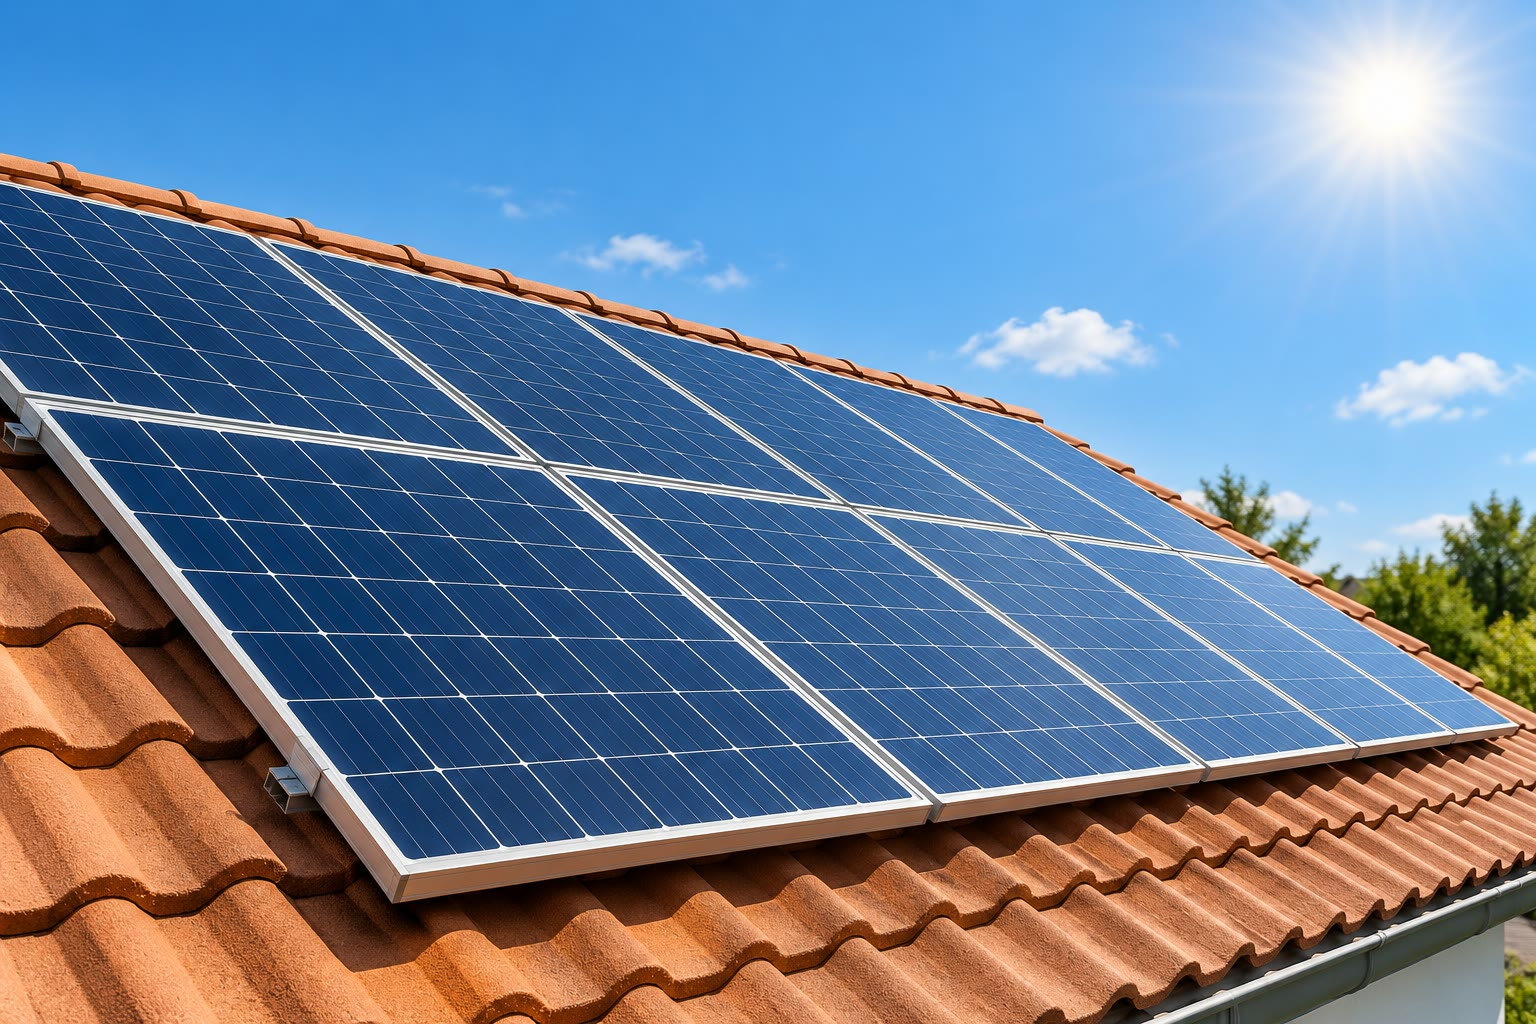
\includegraphics[width=0.6\linewidth]{images/book4/ai/b3-22-solar-panels.jpg}

{\small Zonnepanelen op een pannendak: elke cel is een dun plakje
silicium waarin licht elektronen over een \omterm{def:b3:solid-state:band}{bandkloof} van ongeveer één
elektronvolt tilt.}
\end{omfigure}

\section{Van orbitalen naar banden}

Neem een keten van $N$ identieke atomen, elk met één orbitaal s, in de
benadering van Hückel: coulombintegraal $\alpha$ op elk atoom, resonantie-integraal $\beta < 0$
tussen buren, nul in alle andere gevallen.

\begin{theorem}[Niveaus van een hückelketen]\label{thm:b3:solid-state:chain}
De $N$ moleculaire orbitalen van een lineaire keten van $N$ atomen hebben de energieën
\[
  E_k = \alpha + 2\beta\cos\frac{k\pi}{N + 1}, \qquad k = 1, \dots, N,
\]
met coëfficiënten $c_j^{(k)} \propto \sin\bigl(jk\pi/(N + 1)\bigr)$ op atoom $j$. Als $N \to \infty$ vullen de niveaus het
interval van $\alpha + 2\beta$ tot $\alpha - 2\beta$ dicht op: een band met breedte $4|\beta|$.
\end{theorem}

\begin{proof}
De seculiere vergelijkingen zijn $\beta c_{j-1} + (\alpha - E)c_j + \beta c_{j+1} = 0$ voor $j = 1, \dots, N$, met $c_0 = c_{N+1} = 0$
(daar is geen atoom). Probeer $c_j = \sin(j\theta)$: omdat $\sin((j - 1)\theta) + \sin((j + 1)\theta) = 2\cos\theta\sin(j\theta)$, wordt elke
vergelijking $(\alpha - E + 2\beta\cos\theta)\sin(j\theta) = 0$, dus $E = \alpha + 2\beta\cos\theta$. De voorwaarde $c_0 = 0$ geldt
voor elke $\theta$, en $c_{N+1} = \sin((N + 1)\theta) = 0$ vereist $\theta = k\pi/(N + 1)$; $k = 1, \dots, N$ geeft $N$ verschillende
niveaus (de andere herhalen ze of verdwijnen). Het laagste en het
hoogste zijn
$\alpha \pm 2\beta\cos(\pi/(N + 1))$, die naderen tot $\alpha \pm 2\beta$; de afstand tussen buren is hoogstens
$2|\beta|\pi/(N + 1)$, wat naar nul gaat.
\end{proof}

Voor $N = 2$ geeft de stelling $\alpha \pm \beta$, de orbitalen van het $\pi$-systeem van etheen; voor
$N = 6$ het hexatrieen met open keten. In drie dimensies gebeurt hetzelfde met
elke soort atoomorbitaal: orbitalen s geven een band s, orbitalen p een
band p, en elke band bevat $2N$ elektronen voor $N$ atomen.

\begin{definition}[Banden]\label{def:b3:solid-state:band}
Een \emph{energieband}\index{energieband} van een kristal is een
continu gebied van toegelaten eenelektronenergieën, gevormd uit de
orbitalen van al zijn atomen. Een
\emph{bandkloof}\index{bandkloof} $E_g$ is een energiegebied zonder niveaus tussen twee
banden. In een \omterm{def:b3:solid-state:classes}{halfgeleider} of een \omterm{def:b3:solid-state:classes}{isolator} bij het absolute nulpunt is
de hoogste gevulde band de \emph{valentieband}\index{valentieband} en de
laagste lege de \emph{geleidingsband}\index{geleidingsband}.
\end{definition}

\begin{definition}[Toestandsdichtheid en ferminiveau]\label{def:b3:solid-state:fermi}
De \emph{toestandsdichtheid}\index{toestandsdichtheid} $g(E)$ is het aantal
niveaus per energie-eenheid (en per atoom of per volume-eenheid) in de buurt van de energie $E$.
Het \emph{ferminiveau}\index{ferminiveau} $E_F$ is de energie waarbij een
niveau de waarschijnlijkheid $1/2$ heeft om bezet te zijn; bij het absolute nulpunt zijn alle niveaus eronder
gevuld en alle niveaus erboven leeg.
\end{definition}

\begin{omfigure}
\begin{tikzpicture}
\begin{axis}[width=0.78\linewidth, height=6.2cm, xmin=0.3, xmax=7.6, ymin=-2.3, ymax=2.3,
  axis lines=left, xtick={1,2,3,4,5,6.6}, xticklabels={2,4,8,16,64,$\infty$: $g(E)$},
  xlabel={aantal atomen $N$}, ylabel={$(E - \alpha)/|\beta|$},
  ytick={-2,-1,0,1,2}, tick label style={font=\small}, label style={font=\small}]
\addplot[only marks, mark=-, mark size=7pt, omDef, thick] table[x=col, y=e] {figdata/out/bachelor-3-band-chain.dat};
\addplot[omThm, thick] table[x expr=6.0+0.55*\thisrow{g}, y=e] {figdata/out/bachelor-3-band-chain-b.dat};
\draw[black!40, dashed] (axis cs:0.3,-2) -- (axis cs:7.6,-2);
\draw[black!40, dashed] (axis cs:0.3,2) -- (axis cs:7.6,2);
\draw[<->, black!60] (axis cs:5.6,-2) -- (axis cs:5.6,2) node[midway, left, font=\scriptsize] {$4|\beta|$};
\end{axis}
\end{tikzpicture}

{\small Hückelniveaus van ketens van 2 tot 64 atomen (één kort streepje
per niveau; met $\beta < 0$ liggen de bindende niveaus onderaan). De niveaus dringen samen tot een band
tussen $\alpha + 2\beta$ en $\alpha - 2\beta$; rechts de \omterm{def:b3:solid-state:fermi}{toestandsdichtheid} van de oneindige
keten, het grootst aan de randen van de band.}
\end{omfigure}

\begin{proposition}[Bandvulling]\label{prop:b3:solid-state:filling}
Een kristal waarvan de hoogste bezette band gedeeltelijk gevuld is,
geleidt elektriciteit zoals een metaal; een kristal waarvan de banden
ofwel vol ofwel leeg zijn, met een kloof ertussen, geleidt niet bij het
absolute nulpunt.
\end{proposition}

\begin{proof}[Beargumenteerd]
In een elektrisch veld winnen elektronen een beetje energie en impuls:
ze moeten naar lege niveaus net boven de niveaus die ze bezetten. In een
gedeeltelijk gevulde band liggen zulke niveaus onmiddellijk boven het
\omterm{def:b3:solid-state:fermi}{ferminiveau}, zonder energiekost. In een volle band is elk niveau bezet en
ligt het volgende lege niveau aan de overkant van de kloof; bovendien
draagt een volle band geen netto stroom, omdat er voor elk elektron dat
de ene kant op beweegt een ander de andere kant op beweegt.
\end{proof}

Natrium, met één elektron 3s per atoom, vult zijn band s voor de helft:
een metaal. Magnesium, met twee, zou zijn band s precies vullen, maar de
banden s en p overlappen, zodat ook magnesium een metaal is. Diamant en
silicium hebben vier valentie-elektronen per atoom in orbitalen die
opsplitsen in een gevulde bindende band en een lege antibindende band,
gescheiden door een kloof.

\begin{definition}[Halfgeleiders en isolatoren]\label{def:b3:solid-state:classes}
Een \emph{halfgeleider}\index{halfgeleider} is een vaste stof met een
\omterm{def:b3:solid-state:band}{bandkloof} die klein genoeg is (tot ongeveer \qty{3}{eV}) opdat een meetbaar aantal elektronen
haar oversteekt bij gewone temperatuur of na dotering; een
\emph{isolator}\index{isolator} heeft een kloof die zo groot is dat hij
niet geleidt.
\end{definition}

\begin{omfigure}
\begin{tikzpicture}[font=\small]
  \foreach \x/\name in {0/metaal, 3.6/halfgeleider, 7.2/isolator} {
    \node[font=\small\bfseries] at (\x+0.8,4.3) {\name};
  }
  % metal: one partly filled band
  \fill[omDef!55] (0,0.4) rectangle (1.6,2.0);
  \draw (0,0.4) rectangle (1.6,3.4);
  \draw[omThm, thick] (-0.25,2.0) -- (1.85,2.0) node[right, font=\scriptsize] {$E_F$};
  % semiconductor: small gap
  \fill[omDef!55] (3.6,0.4) rectangle (5.2,1.7);
  \draw (3.6,0.4) rectangle (5.2,1.7);
  \draw (3.6,2.5) rectangle (5.2,3.8);
  \draw[omThm, thick] (3.35,2.1) -- (5.45,2.1) node[right, font=\scriptsize] {$E_F$};
  \draw[<->] (4.4,1.7) -- (4.4,2.5) node[pos=0.8, right, font=\scriptsize] {$E_g$};
  % insulator: large gap
  \fill[omDef!55] (7.2,0.4) rectangle (8.8,1.2);
  \draw (7.2,0.4) rectangle (8.8,1.2);
  \draw (7.2,3.2) rectangle (8.8,4.0);
  \draw[omThm, thick] (6.95,2.2) -- (9.05,2.2) node[right, font=\scriptsize] {$E_F$};
  \draw[<->] (8.0,1.2) -- (8.0,3.2) node[pos=0.75, right, font=\scriptsize] {$E_g$};
  \node[font=\scriptsize, anchor=east] at (3.5,1.05) {valentie};
  \node[font=\scriptsize, anchor=east] at (3.5,3.15) {geleiding};
  \draw[->] (-0.6,0.2) -- (-0.6,3.9) node[above, font=\scriptsize] {$E$};
\end{tikzpicture}

{\small Bandvulling bij het absolute nulpunt (gevulde niveaus gearceerd).
Een metaal heeft een gedeeltelijk gevulde band met zijn \omterm{def:b3:solid-state:fermi}{ferminiveau} erin;
een \omterm{def:b3:solid-state:classes}{halfgeleider} en een \omterm{def:b3:solid-state:classes}{isolator} hebben een volle \omterm{def:b3:solid-state:band}{valentieband} en een
lege \omterm{def:b3:solid-state:band}{geleidingsband}, met het \omterm{def:b3:solid-state:fermi}{ferminiveau} in de kloof, die bij de eerste
smal en bij de tweede breed is.}
\end{omfigure}

\section{Halfgeleiders}

\begin{definition}[Ladingsdragers]\label{def:b3:solid-state:carriers}
Een \emph{intrinsieke halfgeleider}\index{intrinsieke halfgeleider} is een
zuivere \omterm{def:b3:solid-state:classes}{halfgeleider}, waarvan alle ladingsdragers afkomstig zijn van
elektronen die over de kloof aangeslagen zijn. Een
\emph{ladingsdrager}\index{ladingsdrager} is een beweeglijk deeltje dat
stroom draagt: een elektron in de \omterm{def:b3:solid-state:band}{geleidingsband}, of een
\emph{gat}\index{gat}, een leeg niveau in de \omterm{def:b3:solid-state:band}{valentieband}, dat zich
gedraagt als een positieve lading.
\end{definition}

\begin{theorem}[Intrinsieke dragerconcentratie]\label{thm:b3:solid-state:intrinsic}
Met $N_c$ en $N_v$ de effectieve toestandsdichtheden van de geleidings- en de
\omterm{def:b3:solid-state:band}{valentieband} (aangenomen) zijn de elektronen- en gatenconcentraties van
een \omterm{def:b3:solid-state:classes}{halfgeleider} waarvan het \omterm{def:b3:solid-state:fermi}{ferminiveau} meer dan enkele $kT$ van beide bandranden verwijderd is
\[
  n = N_c\,\eu^{-(E_c - E_F)/kT}, \qquad p = N_v\,\eu^{-(E_F - E_v)/kT},
\]
en in een \omterm{def:b3:solid-state:carriers}{intrinsieke halfgeleider}
\[
  n = p = n_i = \sqrt{N_cN_v}\,\eu^{-E_g/2kT}.
\]
\end{theorem}

\begin{proof}
De bezetting van een niveau met energie $E$ is $f(E) = 1/(1 + \eu^{(E - E_F)/kT})$. Als
$E - E_F \gg kT$, is $f \approx \eu^{-(E - E_F)/kT}$, een boltzmannstaart. Optellen over de niveaus van de
\omterm{def:b3:solid-state:band}{geleidingsband} geeft $n = \int g_c(E)\eu^{-(E - E_F)/kT}\,\dd E = \eu^{-(E_c - E_F)/kT}\int g_c(E)\eu^{-(E - E_c)/kT}\,\dd E$, en de laatste integraal is per
definitie $N_c$. \omterm{def:b3:solid-state:carriers}{Gaten} zijn lege niveaus, met waarschijnlijkheid $1 - f \approx \eu^{-(E_F - E)/kT}$ in de
\omterm{def:b3:solid-state:band}{valentieband}; dezelfde stappen geven $p$. Dan is $np = N_cN_v\eu^{-(E_c - E_v)/kT} = N_cN_v\eu^{-E_g/kT}$, en in een zuiver kristal
laat elk aangeslagen elektron één \omterm{def:b3:solid-state:carriers}{gat} achter: $n = p$, dus $n = \sqrt{np}$.
\end{proof}

\begin{proposition}[Massawerkingswet]\label{prop:b3:solid-state:mass-action}
In elke \omterm{def:b3:solid-state:classes}{halfgeleider} in evenwicht, al dan niet gedoteerd, is $np = n_i^2$.
\end{proposition}

\begin{proof}
Het product $np = N_cN_v\eu^{-E_g/kT}$ dat in het bewijs van
\cref{thm:b3:solid-state:intrinsic} gevonden werd, bevat $E_F$ niet: het is hetzelfde, wat het
\omterm{def:b3:solid-state:fermi}{ferminiveau} ook vastlegt, en gelijk aan zijn intrinsieke waarde $n_i^2$. Het is de
evenwichtsconstante van $\text{niets} \rightleftharpoons \mathrm e^- + \mathrm h^+$, zoals het ionenproduct van water.
\end{proof}

\begin{omfigure}
% ledger: eg:Si.E0, eg:Si.a, eg:Si.b, eg:Ge.E0, eg:Ge.a, eg:Ge.b, dos:Si.Nc, dos:Si.Nv, dos:Ge.Nc, dos:Ge.Nv, dop:Si.P
\begin{tikzpicture}
\begin{axis}[name=a, width=0.45\linewidth, height=5.6cm, xmin=1.2, xmax=4.2, ymin=4, ymax=18,
  axis lines=left, xlabel={$1000\,\mathrm K/T$}, ylabel={$\log_{10}(n_i/\unit{cm^{-3}})$},
  tick label style={font=\scriptsize}, label style={font=\small}]
\addplot[omDef, thick] table[x=invT, y=lgSi] {figdata/out/bachelor-3-semiconductor-carriers.dat};
\addplot[omThm, thick] table[x=invT, y=lgGe] {figdata/out/bachelor-3-semiconductor-carriers.dat};
\node[font=\scriptsize, omDef] at (axis cs:3.4,8.3) {Si};
\node[font=\scriptsize, omThm, anchor=south west] at (axis cs:3.4,14.0) {Ge};
\end{axis}
\begin{axis}[at={(a.east)}, anchor=west, xshift=1.7cm, width=0.45\linewidth, height=5.6cm,
  xmin=1, xmax=25, ymin=10, ymax=17, axis lines=left,
  xlabel={$1000\,\mathrm K/T$}, ylabel={$\log_{10}(n/\unit{cm^{-3}})$},
  tick label style={font=\scriptsize}, label style={font=\small}]
\addplot[omDef, thick] table[x=invT, y=lgn] {figdata/out/bachelor-3-semiconductor-carriers-b.dat};
\addplot[black!45, dashed, unbounded coords=jump, restrict y to domain=10:17] table[x=invT, y=lgni] {figdata/out/bachelor-3-semiconductor-carriers-b.dat};
\node[font=\scriptsize, anchor=west] at (axis cs:2.6,16.4) {intrinsiek};
\node[font=\scriptsize] at (axis cs:12,15.35) {verzadiging, $n = N_D$};
\node[font=\scriptsize] at (axis cs:20,13.2) {invriezen};
\end{axis}
\end{tikzpicture}

{\small Links: intrinsieke dragerconcentraties van silicium en germanium
tegen
$1/T$ (model met de gemeten kloven en effectieve toestandsdichtheden); de
hellingen liggen dicht bij $-E_g/2k$. Rechts: elektronen in silicium gedoteerd met
$\qty{1e15}{cm^{-3}}$ fosfor: bij lage temperatuur houden de donoren hun elektronen vast
(invriezen), van ongeveer 150 tot \qty{500}{K} zijn ze allemaal geïoniseerd ($n = N_D$), en bij hoge
temperatuur nemen de intrinsieke dragers (gestreept, $n_i$) het over.}
\end{omfigure}

\begin{definition}[Directe en indirecte kloven]\label{def:b3:solid-state:gap-types}
Een \omterm{def:b3:solid-state:classes}{halfgeleider} heeft een
\emph{directe bandkloof}\index{directe bandkloof} wanneer de top van zijn
\omterm{def:b3:solid-state:band}{valentieband} en de bodem van zijn \omterm{def:b3:solid-state:band}{geleidingsband} bij dezelfde
elektronenimpuls liggen, zodat een foton alleen een elektron kan
overbrengen, en een
\emph{indirecte bandkloof}\index{indirecte bandkloof} wanneer dat niet zo
is, zodat de overgang ook een roostervibratie vereist.
\end{definition}

% ledger: eg:Si, eg:Ge, eg:GaAs, eg:GaN, eg:GaP
Silicium (\qty{1.12}{eV}) en germanium (\qty{0.66}{eV}) hebben indirecte
kloven: in een dikke laag absorberen ze licht goed genoeg, wat geschikt
is voor een zonnecel, maar ze zenden het zeer slecht uit. Galliumarsenide
(\qty{1.42}{eV}) en galliumnitride (ongeveer
\qty{3.4}{eV}) hebben directe kloven, de basis van infrarode en blauwe
lichtgevende diodes en lasers; galliumfosfide (\qty{2.26}{eV}) is
indirect, maar zendt gedoteerd groen licht uit. De kleur van veel
pigmenten is ook een \omterm{def:b3:solid-state:band}{bandkloof}: een kristal
absorbeert alle fotonen met $h\nu > E_g$, zodat cadmiumsulfide, met een kloof in het blauw,
geel is.

\begin{definition}[Dotering]\label{def:b3:solid-state:doping}
Een \emph{doteerstof}\index{doteerstof} is een vreemd atoom dat
opzettelijk en in kleine hoeveelheden in een \omterm{def:b3:solid-state:classes}{halfgeleider} gebracht wordt
om \omterm{def:b3:solid-state:carriers}{ladingsdragers} te leveren. In een
\emph{n-type halfgeleider}\index{n-type halfgeleider} heeft de doteerstof
één valentie-elektron meer dan het atoom dat hij vervangt (fosfor in
silicium) en geeft hij dat af aan de \omterm{def:b3:solid-state:band}{geleidingsband} vanuit een
\emph{donorniveau}\index{donorniveau} net onder die band; in een
\emph{p-type halfgeleider}\index{p-type halfgeleider} heeft hij er één
minder (boor in silicium) en neemt hij een elektron uit de \omterm{def:b3:solid-state:band}{valentieband}
op in een
\emph{acceptorniveau}\index{acceptorniveau} net daarboven, waarbij een \omterm{def:b3:solid-state:carriers}{gat}
achterblijft.
\end{definition}

\begin{omfigure}
\begin{tikzpicture}[font=\small]
  \foreach \x in {0, 5.2} {
    \fill[omDef!35] (\x,0) rectangle (\x+3.6,1.0);
    \fill[omDef!12] (\x,2.6) rectangle (\x+3.6,3.6);
    \node[font=\scriptsize] at (\x+1.8,0.5) {valentieband};
    \node[font=\scriptsize] at (\x+1.8,3.1) {geleidingsband};
  }
  \foreach \i in {0,...,5} { \draw[omThm, thick] (0.25+\i*0.55,2.35) -- (0.6+\i*0.55,2.35); }
  \node[font=\scriptsize, anchor=west] at (0.1,1.95) {donorniveaus, \qty{0.045}{eV} lager};
  \draw[->, omThm] (0.42,2.42) -- (0.42,2.9);
  \fill[omThm] (0.42,2.95) circle (1.6pt);
  \foreach \i in {0,...,5} { \draw[omMeth, thick] (5.45+\i*0.55,1.25) -- (5.8+\i*0.55,1.25); }
  \node[font=\scriptsize, anchor=west] at (5.3,1.6) {acceptorniveaus, \qty{0.045}{eV} hoger};
  \draw[->, omMeth] (5.62,0.7) -- (5.62,1.18);
  \draw[omMeth, fill=white] (5.62,0.62) circle (1.8pt);
  \node[font=\small\bfseries] at (1.8,4.0) {n-type: Si met P};
  \node[font=\small\bfseries] at (7.0,4.0) {p-type: Si met B};
\end{tikzpicture}

{\small Donor- en \omterm{def:b3:solid-state:doping}{acceptorniveaus} in de kloof van silicium (kloof niet op
schaal: de niveaus van de doteerstoffen liggen ongeveer 0.045 eV van de
bandranden, de kloof is 1.12 eV). Een donor geeft zijn elektron (stip)
af aan de \omterm{def:b3:solid-state:band}{geleidingsband}; een acceptor neemt er een op uit de
\omterm{def:b3:solid-state:band}{valentieband} en laat een \omterm{def:b3:solid-state:carriers}{gat} (cirkel) achter.}
\end{omfigure}

% ledger: dop:Si.P, dop:Si.B
Het \omterm{def:b3:solid-state:doping}{donorniveau} van fosfor ligt \qty{0.045}{eV} onder de \omterm{def:b3:solid-state:band}{geleidingsband}
van silicium, minder dan $2kT$ bij kamertemperatuur, en het \omterm{def:b3:solid-state:doping}{acceptorniveau} van boor even
ver boven de \omterm{def:b3:solid-state:band}{valentieband}: bij \qty{300}{K} is bijna elke \omterm{def:b3:solid-state:doping}{doteerstof}
geïoniseerd. Daarom verhoogt
één doteeratoom per $10^7$ siliciumatomen ($\qty{5e15}{cm^{-3}}$) de
elektronenconcentratie enkele honderdduizenden keren.

\begin{method}[Ladingsdragers van een gedoteerde halfgeleider]\label{met:b3:solid-state:doping}
\begin{enumerate}
  \item Controleer dat de temperatuur in het verzadigingsgebied ligt
        (doteerstoffen volledig geïoniseerd, $N_D \gg n_i$): dan zijn de meerderheidsdragers $n \approx N_D$ (of $p \approx N_A$).
  \item Haal de minderheidsdragers uit de massawerkingswet: $p = n_i^2/N_D$.
  \item Plaats het \omterm{def:b3:solid-state:fermi}{ferminiveau}: $E_c - E_F = kT\ln(N_c/n)$, of ten opzichte van het intrinsieke niveau
        $E_F - E_i = kT\ln(n/n_i)$.
  \item Als beide soorten \omterm{def:b3:solid-state:doping}{doteerstof} aanwezig zijn, gebruik dan het verschil $N_D - N_A$.
\end{enumerate}
\end{method}

\begin{definition}[pn-overgang]\label{def:b3:solid-state:junction}
Een \emph{pn-overgang}\index{pn-overgang} is de grens, binnen één
kristal, tussen een p-type en een n-type gebied.
\end{definition}

Aan een \omterm{def:b3:solid-state:junction}{pn-overgang} diffunderen elektronen van de n-kant naar de p-kant
en \omterm{def:b3:solid-state:carriers}{gaten} in de andere richting, wat een dunne laag zonder \omterm{def:b3:solid-state:carriers}{ladingsdragers}
achterlaat waarin de vaste geïoniseerde doteeratomen een elektrisch veld
opbouwen; in evenwicht is het \omterm{def:b3:solid-state:fermi}{ferminiveau} aan beide kanten hetzelfde. Een
spanning in de ene richting verlaagt de barrière en er vloeit stroom; in
de andere richting verhoogt ze haar: een diode. In een lichtgevende
diode recombineren elektronen en \omterm{def:b3:solid-state:carriers}{gaten} die over de overgang
geïnjecteerd worden, en zenden ze fotonen uit met een energie
dicht bij $E_g$; in een zonnecel maken fotonen die dicht bij de overgang
geabsorbeerd worden elektron-gatparen die het veld scheidt, en vloeit er
een stroom in de uitwendige kring.

\begin{omfigure}
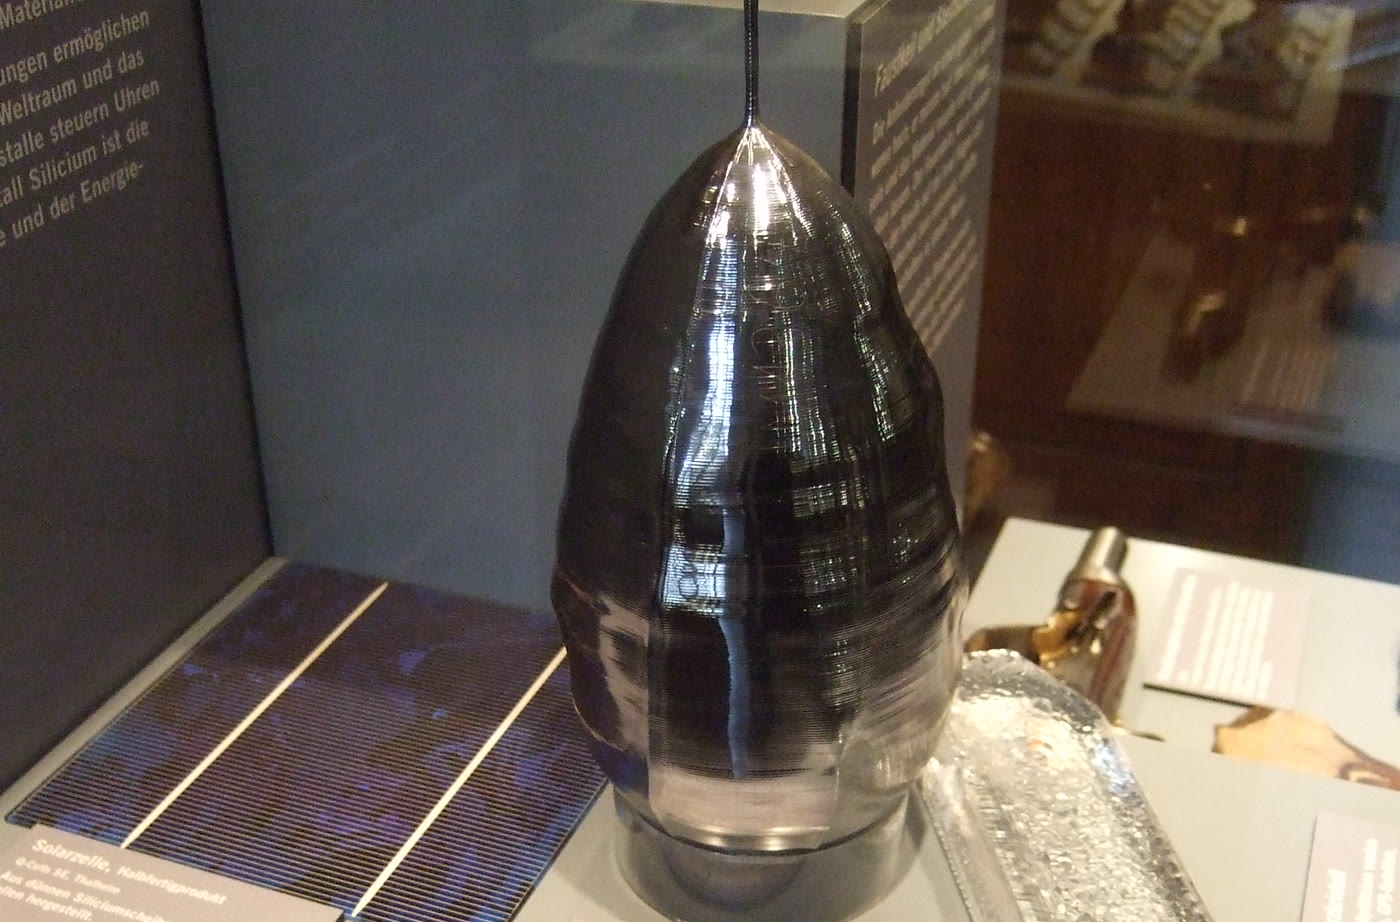
\includegraphics[width=0.5\linewidth]{images/book4/silicon-boule.jpg}

{\small Een éénkristal van silicium, uit de smelt getrokken, naast een
zonnecel die gemaakt is uit een plak van zo'n kristal. Foto: Sebastian
Wallroth, publiek domein.}
\end{omfigure}

\begin{inthelab}[Een siliciumkristal laten groeien]
Bij de methode van Czochralski wordt zeer zuiver polykristallijn
silicium onder argon gesmolten in een smeltkroes van silica, iets boven
zijn smeltpunt, met de \omterm{def:b3:solid-state:doping}{doteerstof} aan de smelt toegevoegd. Een klein
entkristal op een draaiende staaf wordt in de smelt gedompeld en langzaam
opgetrokken: silicium kristalliseert erop met de oriëntatie van het
entkristal, en de trek- en draaisnelheid bepalen de diameter. De
kristalstaaf wordt daarna in wafers van minder dan een millimeter dik
gezaagd. Silaan en de doteergassen fosfine en arsine die in latere
stappen gebruikt worden, zijn pyrofoor of zeer giftig en worden alleen
in gesloten industriële systemen gehanteerd.
\end{inthelab}

\section{Puntdefecten}

\begin{definition}[Puntdefecten]\label{def:b3:solid-state:defects}
Een \emph{puntdefect}\index{puntdefect} is een afwijking van het perfecte
kristal die op één plaats gelokaliseerd is: een vacature, een
interstitieel atoom of een vreemd atoom. In een ionkristal is een
\emph{schottkydefect}\index{schottkydefect} een paar vacatures, één
kation- en één anionvacature, waarbij de ionen naar het oppervlak
verhuisd zijn; een \emph{frenkeldefect}\index{frenkeldefect} is een paar
bestaande uit een vacature en het ion dat haar verlaten heeft en dat op
een interstitiële plaats zit.
\end{definition}

\begin{omfigure}
\begin{tikzpicture}[scale=0.62]
  \begin{scope}
  \foreach \i in {0,...,5} \foreach \j in {0,...,4} {
    \pgfmathtruncatemacro{\pty}{mod(\i+\j,2)}
    \ifnum\pty=0 \fill[omDef!70] (\i,\j) circle (0.2); \else \fill[omThm!25] (\i,\j) circle (0.38); \draw[omThm!60] (\i,\j) circle (0.38); \fi
  }
  \fill[white] (2,2) circle (0.45); \draw[dashed] (2,2) circle (0.3);
  \fill[white] (3,2) circle (0.45); \draw[dashed] (3,2) circle (0.38);
  \node[font=\small\bfseries] at (2.5,5.0) {Schottky (NaCl)};
  \end{scope}
  \begin{scope}[xshift=8cm]
  \foreach \i in {0,...,5} \foreach \j in {0,...,4} {
    \pgfmathtruncatemacro{\pty}{mod(\i+\j,2)}
    \ifnum\pty=0 \fill[black!45] (\i,\j) circle (0.2); \else \fill[omMeth!25] (\i,\j) circle (0.38); \draw[omMeth!60] (\i,\j) circle (0.38); \fi
  }
  \fill[white] (2,2) circle (0.3); \draw[dashed] (2,2) circle (0.22);
  \fill[black!45] (2.5,2.5) circle (0.2);
  \draw[->, thick] (2.1,2.1) -- (2.38,2.38);
  \node[font=\small\bfseries] at (2.5,5.0) {Frenkel (AgCl)};
  \end{scope}
\end{tikzpicture}

{\small \omterm{def:b3:solid-state:defects}{Puntdefecten} in een laag van een kristal met steenzoutstructuur
(kleine stippen: kationen; grote cirkels: anionen; gestreept: vacatures).
Links: een schottkypaar, één kation en één anion ontbreken. Rechts: een
frenkelpaar, een zilverion dat van zijn plaats naar een interstitiële
positie verhuisd is.}
\end{omfigure}

\begin{theorem}[Evenwichtsconcentratie van schottkydefecten]\label{thm:b3:solid-state:schottky}
In een kristal MX van $N$ formule-eenheden is het aantal $n$ schottkyparen in
evenwicht, met vormingsenthalpie $\Delta H_S$ per paar en $n \ll N$,
\[
  \frac{n}{N} = \eu^{-\Delta H_S/2kT}.
\]
\end{theorem}

\begin{proof}
Het maken van $n$ paren kost $n\,\Delta H_S$ en levert een configuratie-entropie op, uit de
$\binom{N}{n}$ manieren om de kationvacatures te kiezen en evenveel voor de anionen:
$S = 2k\ln\frac{N!}{n!(N - n)!}$. Met de formule van Stirling $\ln x! \approx x\ln x - x$ is
\[
  G(n) = n\,\Delta H_S - 2kT\bigl[N\ln N - n\ln n - (N - n)\ln(N - n)\bigr].
\]
In evenwicht is $\dd G/\dd n = 0$: $\Delta H_S - 2kT\ln\frac{N - n}{n} = 0$, dus $n/(N - n) = \eu^{-\Delta H_S/2kT}$, en $n/N$ voor
$n \ll N$. De vibratie-entropie van de defecten, hier verwaarloosd,
vermenigvuldigt het resultaat met een constante factor.
\end{proof}

\begin{proposition}[Frenkeldefecten]\label{prop:b3:solid-state:frenkel}
Met $N$ ionen van de beweeglijke soort, $N_i$ interstitiële plaatsen die voor hen beschikbaar zijn en
$\Delta H_F$ de vormingsenthalpie van een paar is het aantal frenkelparen $n =
\sqrt{NN_i}\,\eu^{-\Delta H_F/2kT}$ (voor $n \ll N, N_i$).
\end{proposition}

\begin{proof}
De entropie is nu $S = k\ln\binom{N}{n} + k\ln\binom{N_i}{n}$, en dezelfde minimalisatie geeft
\[
  \Delta H_F = kT\ln\frac{(N - n)(N_i - n)}{n^2} \approx kT\ln\frac{NN_i}{n^2},
\]
waaruit het resultaat volgt.
\end{proof}

De vierkantswortel toont dat defecten in paren ontstaan: zoals $n_i$ in een \omterm{def:b3:solid-state:classes}{halfgeleider}
heeft hun concentratie de helft van de vormingsenergie in haar exponent.
Alkalihalogeniden vormen vooral \omterm{def:b3:solid-state:defects}{schottkydefecten}; zilverhalogeniden,
waarvan het kleine, polariseerbare
$\ce{Ag+}$ tussen de anionen past, vooral \omterm{def:b3:solid-state:defects}{frenkeldefecten}.

\begin{definition}[Notatie van Kröger-Vink]\label{def:b3:solid-state:kroger-vink}
De \emph{notatie van Kröger-Vink}\index{notatie van Kroger-Vink@notatie van Kröger-Vink}
schrijft een \omterm{def:b3:solid-state:defects}{puntdefect} als $\mathrm{A_S^c}$: A is de species op de plaats (V voor een vacature, $i$ als plaats
voor een interstitieel), S de plaats die het in het perfecte kristal
inneemt, en c zijn lading ten opzichte van die plaats: $\bullet$ voor elke positieve eenheid, $'$ voor elke negatieve
eenheid, $\times$ voor geen.
\end{definition}

Zo is $\mathrm{V_{Na}'}$ een natriumvacature (de ontbrekende $+1$ laat een relatieve lading $-1$ achter),
$\mathrm{V_{Cl}^{\bullet}}$ een chloridevacature, $\mathrm{Ag_i^{\bullet}}$ een interstitieel zilverion, $\mathrm{Ca_{Na}^{\bullet}}$ een calciumion op een
natriumplaats, $\mathrm{O_O^{\times}}$ een oxide-ion op zijn plaats. Het schottkyevenwicht van NaCl is
$\text{nul} \rightleftharpoons \mathrm{V_{Na}' + V_{Cl}^{\bullet}}$, het frenkelevenwicht van AgCl
$\mathrm{Ag_{Ag}^{\times}} \rightleftharpoons \mathrm{Ag_i^{\bullet} + V_{Ag}'}$.

\begin{method}[Een defectvergelijking schrijven]\label{met:b3:solid-state:kroger-vink}
\begin{enumerate}
  \item Schrijf op wat aan het gastrooster toegevoegd wordt en welke
        defecten het maakt.
  \item Plaatsbalans: de verhouding van kation- tot anionplaatsen van het
        gastrooster blijft behouden (vacatures tellen als plaatsen).
  \item Massabalans: dezelfde atomen aan beide kanten (vacatures hebben
        geen massa;
        elektronen $e'$ en \omterm{def:b3:solid-state:carriers}{gaten} $h^\bullet$ evenmin).
  \item Ladingsbalans: de sommen van de effectieve ladingen zijn gelijk.
\end{enumerate}
\end{method}

\begin{example}[Yttriumoxide in zirkoniumoxide]
Het oplossen van $\ce{Y2O3}$ in $\ce{ZrO2}$ zet twee $\ce{Y^3+}$ op plaatsen van $\ce{Zr^4+}$, elk met relatieve lading $-1$, en
drie oxide-ionen op zuurstofplaatsen; de verhouding van het gastrooster,
één kation op twee zuurstofplaatsen, vereist vier zuurstofplaatsen voor
de twee kationen, zodat er één leeg blijft:
\[
  \ce{Y2O3} \xrightarrow{\ce{ZrO2}} \mathrm{2\,Y_{Zr}' + 3\,O_O^{\times} + V_O^{\bullet\bullet}}.
\]
Plaatsen: 2 kation, 4 zuurstof; massa: 2 Y en 3 O; lading: $2(-1) + 2 = 0$. Eén
oxidevacature per twee yttriumionen: dat maakt van met yttriumoxide
gestabiliseerd zirkoniumoxide een geleider van oxide-ionen.
\end{example}

\begin{definition}[Kleurcentrum]\label{def:b3:solid-state:colour-centre}
Een \emph{kleurcentrum}\index{kleurcentrum} is een \omterm{def:b3:solid-state:defects}{puntdefect} dat
zichtbaar licht absorbeert, zoals een elektron dat gevangen zit in een
anionvacature van een alkalihalogenide (een F-centrum), wat een kristal
kleurt dat anders doorzichtig is.
\end{definition}

Natriumchloride verhitten in natriumdamp of bestralen maakt F-centra: het
gevangen elektron gedraagt zich als een \omterm{def:b3:quantum-model-systems:box}{deeltje in een doos} ter grootte
van de vacature, en absorbeert in het zichtbare, waardoor het kristal
geelbruin wordt.

\section{Niet-stoichiometrie}

\begin{definition}[Niet-stoichiometrische verbindingen]\label{def:b3:solid-state:non-stoichiometric}
Een \emph{niet-stoichiometrische verbinding}\index{niet-stoichiometrische verbinding}
is een vaste stof waarvan de samenstelling varieert over een gebied rond
een eenvoudige verhouding van gehele getallen, waarbij het verschil
opgevangen wordt door \omterm{def:b3:solid-state:defects}{puntdefecten}.
\end{definition}

IJzer(II)oxide is nooit precies $\ce{FeO}$: het heeft altijd een tekort aan ijzer,
$\mathrm{Fe_{1-x}O}$, met $x$ bepaald door de temperatuur en de zuurstofdruk waarbij het gemaakt werd. Elk ontbrekend $\ce{Fe^2+}$ wordt gecompenseerd door twee
$\ce{Fe^3+}$, die in de taal van de defecten \omterm{def:b3:solid-state:carriers}{gaten} op ijzerplaatsen zijn.

\begin{proposition}[Geleidbaarheid en zuurstofdruk]\label{prop:b3:solid-state:brouwer}
Voor een oxide met metaaltekort $\mathrm{M_{1-x}O}$ waarvan de defecten tweevoudig geladen metaalvacatures zijn,
gecompenseerd door \omterm{def:b3:solid-state:carriers}{gaten}, variëren de gatenconcentratie en de
geleidbaarheid als
$p(\ce{O2})^{1/6}$. Voor een oxide met zuurstoftekort, gecompenseerd door elektronen, variëren ze als
$p(\ce{O2})^{-1/6}$.
\end{proposition}

\begin{proof}
Het opnemen van zuurstof maakt metaalvacatures:
\[
  \tfrac12\ce{O2} \rightleftharpoons \mathrm{O_O^{\times} + V_M'' + 2\,h^{\bullet}}, \qquad K = \frac{[\mathrm{V_M''}][\mathrm h^\bullet]^2}{p(\ce{O2})^{1/2}}
\]
(de activiteit van $\mathrm{O_O^{\times}}$ is 1). De
ladingsbalans is $[\mathrm h^\bullet] = 2[\mathrm{V_M''}]$, dus $[\mathrm h^\bullet]^3 = 2K\,p(\ce{O2})^{1/2}$ en $[\mathrm h^\bullet] \propto p(\ce{O2})^{1/6}$. Voor het
geval met zuurstoftekort is $\mathrm{O_O^{\times}} \rightleftharpoons \tfrac12\ce{O2} + \mathrm{V_O^{\bullet\bullet} + 2\,e'}$, $[\mathrm e'] = 2[\mathrm{V_O^{\bullet\bullet}}]$, en dezelfde stappen geven $[\mathrm e'] \propto p(\ce{O2})^{-1/6}$.
De geleidbaarheid is evenredig met de dragerconcentratie.
\end{proof}

Een grafiek van $\log\sigma$ tegen $\log p(\ce{O2})$ vertelt dus welke defecten overheersen: haar helling,
$\pm 1/4$ of $\pm 1/6$, hangt af van hun ladingen.

\section{Ionengeleiders}

\begin{definition}[Ionengeleiders]\label{def:b3:solid-state:ionic-conductor}
Een \emph{ionengeleider}\index{ionengeleider} is een vaste stof waarin de
stroom gedragen wordt door ionen die door het rooster bewegen. Een
\emph{vaste elektrolyt}\index{vaste elektrolyt} is een ionengeleider
waarvan de elektronische geleidbaarheid verwaarloosbaar is, zodat hij de
twee elektroden van een elektrochemische cel kan scheiden.
\end{definition}

\begin{proposition}[Wet van Arrhenius voor ionengeleiding]\label{prop:b3:solid-state:ionic-arrhenius}
Voor ionen die zich bewegen door te springen tussen naburige plaatsen
over een barrière $E_a$ is
$\sigma T = A\,\eu^{-E_a/kT}$.
\end{proposition}

\begin{proof}[Gedeeltelijk bewijs]
Een ion probeert te springen met een frequentie $\nu_0$ en slaagt met waarschijnlijkheid $\eu^{-E_a/kT}$,
zodat zijn diffusiecoëfficiënt $D = \tfrac16\nu_0 z a^2\eu^{-E_a/kT}$ is voor $z$ naburige plaatsen op
afstand $a$ (toevalswandeling). De betrekking van Nernst-Einstein $\sigma = nq^2D/kT$ (aangenomen), voor $n$
beweeglijke ionen met lading $q$ per volume-eenheid, geeft $\sigma T = (nq^2\nu_0za^2/6k)\,\eu^{-E_a/kT}$. De
concentratie $n$ ligt vast door dotering in een extrinsieke geleider;
als ze zelf thermisch ontstaat, bevat $E_a$ ook de helft van de vormingsenthalpie.
\end{proof}

% ledger: trans:AgI
Drie \omterm{def:b3:solid-state:ionic-conductor}{vaste elektrolyten} tonen de verscheidenheid. In met yttriumoxide
gestabiliseerd zirkoniumoxide laten de oxidevacatures die de \omterm{def:b3:solid-state:doping}{doteerstof}
maakt, ionen $\ce{O^2-}$ springen; het geleidt alleen nuttig
als het heet is, bij enkele honderden graden Celsius. In $\beta$-aluminiumoxide bewegen natriumionen in
losgepakte vlakken tussen spinelblokken, de basis van
natrium-zwavelbatterijen. Zilverjodide wordt boven \qty{146}{\celsius} een
superionische geleider, waarbij zijn zilverionen verdeeld zijn over
veel meer plaatsen dan er ionen zijn, bijna als een vloeistof binnen een
star jodiderooster. Lithiumionengeleiders (granaten van
lithiumlanthaanzirkonaat, sulfiden) zijn de elektrolyten van de
volledig vaste batterijen die nu ontwikkeld worden.

\begin{omfigure}
\begin{tikzpicture}[font=\small, >=Stealth]
  \fill[omProp!25] (0,0) rectangle (2.4,3.2);
  \node[font=\scriptsize, align=center] at (1.2,0.6) {$\ce{ZrO2}$--$\ce{Y2O3}$\\ vaste elektrolyt};
  \draw[black!60, line width=2.5pt] (-0.07,0) -- (-0.07,3.2);
  \draw[black!60, line width=2.5pt] (2.47,0) -- (2.47,3.2);
  \node[font=\scriptsize, align=center] at (-2.0,1.4) {uitlaatgas\\ $p(\ce{O2})$ laag};
  \node[font=\scriptsize, align=center] at (4.4,1.4) {referentielucht\\ $p(\ce{O2}) = \qty{0.21}{bar}$};
  \node[font=\scriptsize, anchor=north] at (-0.07,-0.05) {Pt};
  \node[font=\scriptsize, anchor=north] at (2.47,-0.05) {Pt};
  \draw[->, thick, omThm] (2.0,1.9) -- (0.4,1.9) node[midway, above, font=\scriptsize] {$\ce{O^2-}$};
  \node[font=\scriptsize, anchor=west] at (2.65,2.75) {$\ce{O2 + 4e- -> 2O^2-}$};
  \node[font=\scriptsize, anchor=east] at (-0.25,2.75) {$\ce{2O^2- -> O2 + 4e-}$};
  \draw (-0.07,3.2) -- (-0.07,4.0) -- (0.85,4.0);
  \draw (2.47,3.2) -- (2.47,4.0) -- (1.55,4.0);
  \draw (1.2,4.0) circle (0.35) node {V};
\end{tikzpicture}

{\small De zirkoniumoxidezuurstofsensor in doorsnede: poreuze
platina-elektroden op de twee vlakken van de \omterm{def:b3:solid-state:ionic-conductor}{vaste elektrolyt}, één in de
uitlaat en één in de lucht. Oxide-ionen dragen de stroom door de
elektrolyt; de spanning meet de verhouding van de twee zuurstofdrukken.}
\end{omfigure}

\begin{history}[De transistor en het getrokken kristal]
In 1947 maakten John Bardeen en Walter Brattain, in de groep van William
Shockley bij Bell Laboratories, de eerste transistor uit een kristal van
germanium; de drie deelden de Nobelprijs voor de Natuurkunde van 1956.
De kristallen kwamen van een methode die Jan Czochralski in 1916 gevonden
had toen hij mat hoe snel metalen kristalliseren, door een draad tin uit
de smelt te trekken: aangepast aan germanium en daarna aan silicium,
maakt ze nog steeds de wafers van bijna alle geïntegreerde schakelingen.
\end{history}

\section{Oefeningen}

\begin{exercise}[$\star$]\label{exo:b3:solid-state:1}
Geef de zes hückelniveaus van een keten van zes atomen in eenheden $|\beta|$, en de
breedte van het gebied dat ze bestrijken.
\end{exercise}

\begin{exercise}[$\star$]\label{exo:b3:solid-state:2}
Hoeveel elektronen bevat een band die opgebouwd is uit de orbitalen s
van $N$ atomen? Waarom
zijn natrium en magnesium allebei metalen?
\end{exercise}

\begin{exercise}[$\star$]\label{exo:b3:solid-state:3}
Schat de golflengte van het licht dat uitgezonden wordt door diodes van
galliumfosfide
(\qty{2.26}{eV}) en galliumnitride (\qty{3.4}{eV}), met $\lambda \approx hc/E_g$.
\end{exercise}

\begin{exercise}[$\star$]\label{exo:b3:solid-state:4}
Schrijf de vergelijkingen van Kröger-Vink op voor het oplossen van $\ce{CaCl2}$ in $\ce{NaCl}$ en van $\ce{Y2O3}$ in $\ce{ZrO2}$, en
controleer elke balans.
\end{exercise}

\begin{exercise}[$\star\star$]\label{exo:b3:solid-state:5}
Bereken met $N_c = \num{6.2e15}\,T^{3/2}$, $N_v = \num{3.5e15}\,T^{3/2}$ (in $\unit{cm^{-3}}$) en $E_g = \qty{1.125}{eV}$ voor silicium bij \qty{300}{K},
en $N_c = \num{1.98e15}\,T^{3/2}$, $N_v = \num{9.6e14}\,T^{3/2}$, $E_g = \qty{0.661}{eV}$ voor germanium, $n_i$ voor elk, en hun
verhouding.
\end{exercise}

\begin{exercise}[$\star\star$]\label{exo:b3:solid-state:6}
Silicium wordt gedoteerd met $\qty{1.0e16}{cm^{-3}}$ fosfor. Geef met $n_i = \qty{1.0e10}{cm^{-3}}$ bij \qty{300}{K} de
elektronen- en gatenconcentratie.
\end{exercise}

\begin{exercise}[$\star\star$]\label{exo:b3:solid-state:7}
Hoe ver ligt voor het kristal van \cref{exo:b3:solid-state:6} het
\omterm{def:b3:solid-state:fermi}{ferminiveau} boven het intrinsieke niveau?
\end{exercise}

\begin{exercise}[$\star\star$]\label{exo:b3:solid-state:8}
De vormingsenthalpie van een schottkypaar in NaCl is ongeveer \qty{2.3}{eV} (gegevens van de
oefening). Bereken de fractie lege plaatsen bij \qty{800}{K}, en het
aantal paren in een mol.
\end{exercise}

\begin{exercise}[$\star\star$]\label{exo:b3:solid-state:9}
Een monster ijzer(II)oxide (steenzoutstructuur, vier zuurstofplaatsen per
cel) heeft
$a = \qty{430.0}{pm}$ en een dichtheid van \qty{5.70}{g.cm^{-3}} (gegevens van de oefening). Neem
aan dat de zuurstofplaatsen vol zijn en bepaal $x$ in $\mathrm{Fe_{1-x}O}$.
\end{exercise}

\begin{exercise}[$\star\star\star$]\label{exo:b3:solid-state:10}
Een lithiumionengeleider heeft $\sigma = \qty{1.0e-4}{S.cm^{-1}}$ bij \qty{300}{K}, $\qty{7.8e-4}{S.cm^{-1}}$ bij \qty{350}{K} en
$\qty{3.6e-3}{S.cm^{-1}}$ bij \qty{400}{K} (gegevens van de oefening). Bepaal zijn activeringsenergie.
\end{exercise}

\begin{exercise}[$\star\star\star$]\label{exo:b3:solid-state:11}
Toon aan dat in een oxide waarvan de overheersende defecten eenvoudig
geladen metaalvacatures
$\mathrm{V_M'}$ zijn, gecompenseerd door \omterm{def:b3:solid-state:carriers}{gaten}, de geleidbaarheid varieert als $p(\ce{O2})^{1/4}$.
\end{exercise}

\begin{exercise}[$\star\star\star$]\label{exo:b3:solid-state:12}
In AgCl heeft het frenkelpaar een vormingsenthalpie van ongeveer \qty{1.4}{eV}, en zijn er
twee interstitiële plaatsen per zilverion (gegevens van de oefening).
Bereken de fractie
zilverionen op interstitiële plaatsen bij \qty{600}{K}.
\end{exercise}

\section{Probleem: de zuurstofsensor in een uitlaatpijp}

\begin{problem}[{Weekendprobleem --- de zuurstofsensor in een uitlaatpijp:
de defecten van met yttriumoxide gestabiliseerd zirkoniumoxide, zijn
ionengeleidbaarheid en werktemperatuur, de nernstspanning van de cel, en
de omslag tussen arm en rijk uitlaatgas}]
\label{pb:b3:solid-state:1}
% ledger: const:R, const:F, const:kB, const:e, const:NA, air:O2
De elektrolyt van de sensor is zirkoniumoxide met 8.0\,mol\,\% $\ce{Y2O3}$, met fluorietstructuur
met vier kation- en acht zuurstofplaatsen per kubische cel, $a = \qty{514}{pm}$; een schijf
van \qty{1.0}{mm} dik en \qty{0.20}{cm^2} groot scheidt het uitlaatgas van
de lucht. Zijn
geleidbaarheid volgt $\sigma T = A\eu^{-E_a/kT}$ met $E_a = \qty{1.0}{eV}$ en $\sigma = \qty{0.030}{S.cm^{-1}}$ bij \qty{800}{\celsius}. Arm
uitlaatgas heeft $p(\ce{O2}) = \qty{0.010}{bar}$, rijk uitlaatgas $p(\ce{O2}) = \qty{1.0e-20}{bar}$ (alle gegevens van het probleem).

\medskip\noindent\textbf{Deel I --- De elektrolyt.}
\begin{enumerate}
  \item Schrijf de vergelijking van Kröger-Vink op voor het oplossen van $\ce{Y2O3}$ in $\ce{ZrO2}$.
  \item Controleer haar plaats-, massa- en ladingsbalans.
  \item Hoeveel oxidevacatures ontstaan er per yttriumion?
  \item Schrijf de samenstelling als $\mathrm{Zr_{1-x}Y_xO_{2-x/2}}$ en bereken $x$.
  \item Bereken de fractie van de zuurstofplaatsen die leeg is.
  \item Bereken het aantal vacatures per cel.
  \item Bereken de vacatureconcentratie in $\unit{cm^{-3}}$.
\end{enumerate}

\medskip\noindent\textbf{Deel II --- Geleidbaarheid en temperatuur.}
\begin{enumerate}[resume]
  \item Waarom stijgt de geleidbaarheid steil met de temperatuur?
  \item Bereken $A$.
  \item Bereken $\sigma$ bij \qty{700}{\celsius}.
  \item Bereken $\sigma$ bij \qty{300}{\celsius}.
  \item Bereken de weerstand van de schijf bij deze twee temperaturen.
  \item De elektronica vereist een weerstand onder \qty{1}{k\ohm}: bepaal
        de laagste werktemperatuur.
  \item Waarom worden zulke sensoren met een verwarmingselement uitgerust?
\end{enumerate}

\medskip\noindent\textbf{Deel III --- De nernstspanning.}
\begin{enumerate}[resume]
  \item Schrijf de elektrodereactie aan de luchtkant op, in gewone notatie
        en in de \omterm{def:b3:solid-state:kroger-vink}{notatie van Kröger-Vink}.
  \item Toon aan dat de celspanning $E = (RT/4F)\ln\bigl(p_{\mathrm{lucht}}/p_{\mathrm{uitl}}\bigr)$ is.
  \item Bereken $RT/4F$ bij \qty{700}{\celsius}.
  \item Wat is de spanning als het uitlaatgas lucht bevatte?
  \item Bereken de verandering van de spanning per factor tien in $p(\ce{O2})$.
\end{enumerate}

\medskip\noindent\textbf{Deel IV --- Arm, rijk en de omslag.}
\begin{enumerate}[resume]
  \item Bereken de spanning in arm uitlaatgas bij \qty{700}{\celsius}.
  \item Bereken de spanning in rijk uitlaatgas bij \qty{700}{\celsius}.
  \item Waarom is $p(\ce{O2})$ zo klein in rijk uitlaatgas?
  \item De motorsturing schakelt om bij \qty{0.45}{V}: met welke zuurstofdruk komt dat overeen?
  \item Waarom springt de spanning bij de stoichiometrische
        lucht-brandstofverhouding, en hoe gebruikt de motorsturing dat?
  \item Formuleer het resultaat: de spanning van de sensor in rijk
        uitlaatgas bij \qty{700}{\celsius}.
\end{enumerate}
\end{problem}
